% 图 39.1 —— 由 `checks/emit_hand.py` 自动拼出（probe 精测 + prims2 图元分解）
%%
% ⚠ 这是**稿子不是成品**：跑 `checks/checkhand.py 39.1` 看指标 + 看叠合图。
%%
%% ⚠ 待核：
%   · 本图 probe 报出阴影族 2 个 —— **本脚本不生成阴影**（要照原书手写）；prims2 的 strokes 里可能含阴影线，核对时留意别画重
%   · 可疑字形 3 项（空心圈 ⊙ 常被认成字母 o）—— 见文件末
%%
\documentclass[12pt]{standalone}
\usepackage{fontspec}
\setsansfont{Arial}
\newfontfamily\mfallback{DejaVu Sans}
\usepackage{tikz}
\begin{document}
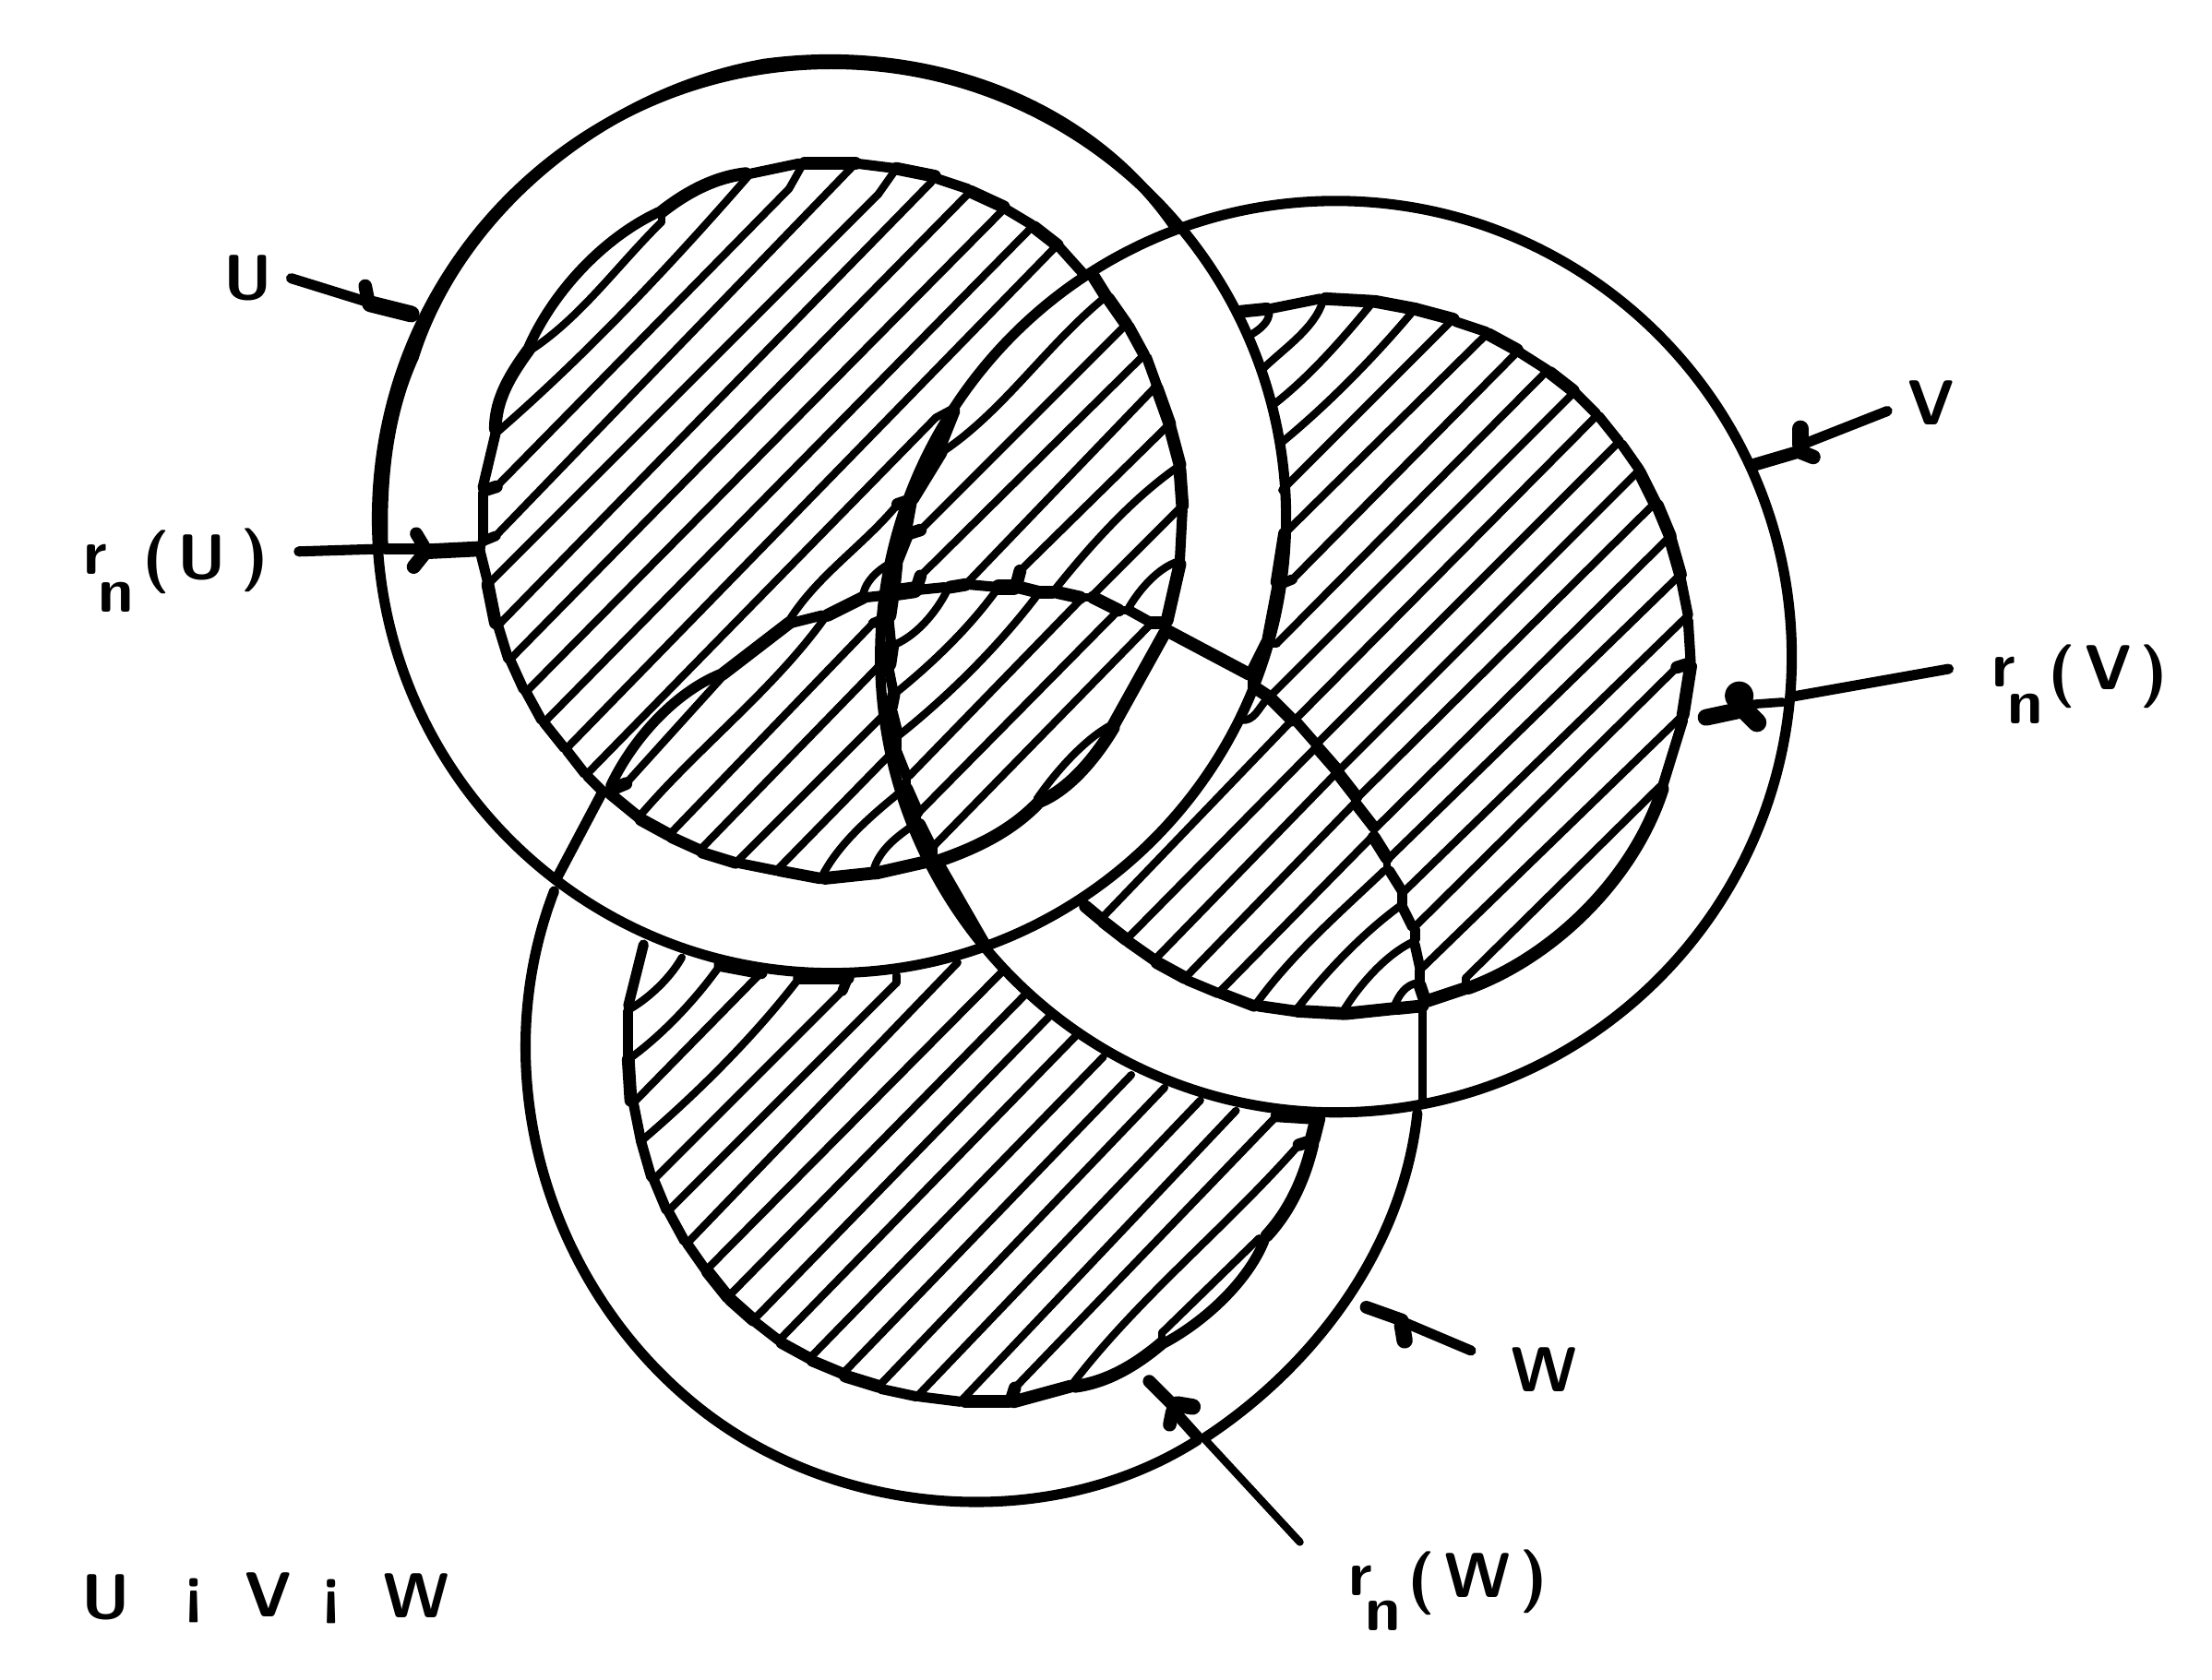
\begin{tikzpicture}[x=1pt, y=-1pt, line width=4.0pt, line cap=round, line join=round]

  %% ════ 填充区（prims2 的 fills）════

  %% ════ 直线段（prims2 的 strokes）════
  \draw[line width=3.0pt] (197.0,260.0) -- (382.0,73.0);
  \draw[line width=6.5pt] (341.0,222.0) -- (348.0,221.0);
  \draw[line width=5.0pt] (652.0,251.0) -- (649.0,270.0);
  \draw[line width=4.0pt] (384.0,72.0) -- (394.0,78.0);
  \draw[line width=4.0pt] (338.0,233.0) -- (339.0,243.0);
  \draw[line width=5.0pt] (341.0,211.0) -- (340.0,221.0);
  \draw[line width=3.0pt] (249.0,77.0) -- (249.0,74.0);
  \draw[line width=4.5pt] (432.0,359.0) -- (442.0,366.0);
  \draw[line width=3.0pt] (345.0,298.0) -- (345.0,295.0);
  \draw[line width=4.0pt] (341.0,279.0) -- (341.0,283.0);
  \draw[line width=5.0pt] (446.0,234.0) -- (441.0,234.0);
  \draw[line width=5.0pt] (694.0,167.0) -- (677.0,172.0);
  \draw[line width=3.0pt] (418.0,223.0) -- (452.0,189.0);
  \draw[line width=3.0pt] (252.0,464.0) -- (341.0,375.0);
  \draw[line width=3.0pt] (341.0,375.0) -- (341.0,372.0);
  \draw[line width=3.0pt] (513.0,293.0) -- (443.0,365.0);
  \draw[line width=5.0pt] (452.0,172.0) -- (448.0,157.0);
  \draw[line width=3.0pt] (276.0,497.0) -- (391.0,380.0);
  \draw[line width=5.0pt] (447.0,237.0) -- (479.0,254.0);
  \draw[line width=5.0pt] (584.0,127.0) -- (573.0,121.0);
  \draw[line width=4.0pt] (350.0,221.0) -- (360.0,220.0);
  \draw[line width=4.0pt] (487.0,111.0) -- (507.0,107.0);
  \draw[line width=4.0pt] (104.0,99.0) -- (133.0,108.0);
  \draw[line width=4.0pt] (572.0,120.0) -- (560.0,116.0);
  \draw[line width=4.0pt] (544.0,360.0) -- (546.0,369.0);
  \draw[line width=5.0pt] (385.0,539.0) -- (368.0,539.0);
  \draw[line width=4.5pt] (459.0,553.0) -- (450.0,543.0);
  \draw[line width=4.0pt] (441.0,234.0) -- (432.0,229.0);
  \draw[line width=3.0pt] (441.0,234.0) -- (356.0,321.0);
  \draw[line width=6.5pt] (151.0,113.0) -- (135.0,109.0);
  \draw[line width=5.0pt] (533.0,326.0) -- (528.0,318.0);
  \draw[line width=4.0pt] (347.0,187.0) -- (345.0,198.0);
  \draw[line width=5.0pt] (443.0,142.0) -- (448.0,156.0);
  \draw[line width=5.0pt] (418.0,98.0) -- (423.0,106.0);
  \draw[line width=5.0pt] (362.0,220.0) -- (368.0,219.0);
  \draw[line width=4.0pt] (648.0,216.0) -- (651.0,231.0);
  \draw[line width=5.0pt] (389.0,220.0) -- (397.0,222.0);
  \draw[line width=4.0pt] (181.0,218.0) -- (178.0,206.0);
  \draw[line width=5.0pt] (339.0,267.0) -- (340.0,262.0);
  \draw[line width=5.0pt] (349.0,308.0) -- (345.0,299.0);
  \draw[line width=3.0pt] (220.0,293.0) -- (356.5,153.5);
  \draw[line width=3.0pt] (356.5,153.5) -- (363.0,150.0);
  \draw[line width=5.5pt] (152.0,212.0) -- (156.0,207.0);
  \draw[line width=5.0pt] (452.0,211.0) -- (447.0,233.0);
  \draw[line width=5.0pt] (333.0,332.0) -- (355.0,327.0);
  \draw[line width=3.0pt] (355.0,61.0) -- (186.0,234.0);
  \draw[line width=5.0pt] (516.0,387.0) -- (498.0,386.0);
  \draw[line width=5.0pt] (325.0,54.0) -- (305.0,54.0);
  \draw[line width=4.0pt] (325.0,54.0) -- (341.0,56.0);
  \draw[line width=3.0pt] (325.0,54.0) -- (184.1,199.9);
  \draw[line width=4.0pt] (184.1,199.9) -- (179.0,202.0);
  \draw[line width=3.0pt] (445.0,515.0) -- (445.0,512.0);
  \draw[line width=3.0pt] (445.0,512.0) -- (483.0,475.0);
  \draw[line width=3.0pt] (190.0,248.0) -- (369.0,66.0);
  \draw[line width=4.0pt] (242.0,360.0) -- (236.0,384.0);
  \draw[line width=3.0pt] (492.0,182.0) -- (558.0,116.0);
  \draw[line width=5.0pt] (288.0,371.0) -- (272.0,368.0);
  \draw[line width=3.0pt] (288.0,371.0) -- (239.0,421.0);
  \draw[line width=3.0pt] (623.0,164.0) -- (506.0,281.0);
  \draw[line width=4.5pt] (229.0,301.0) -- (240.0,310.0);
  \draw[line width=4.5pt] (483.0,384.0) -- (497.0,386.0);
  \draw[line width=4.0pt] (366.0,539.0) -- (350.0,537.0);
  \draw[line width=6.3pt] (457.0,541.0) -- (451.0,540.0);
  \draw[line width=3.0pt] (382.0,371.0) -- (267.0,487.0);
  \draw[line width=5.0pt] (402.0,222.0) -- (397.0,222.0);
  \draw[line width=5.0pt] (321.0,529.0) -- (334.0,533.0);
  \draw[line width=5.0pt] (549.0,382.0) -- (564.0,377.0);
  \draw[line width=4.9pt] (503.0,437.0) -- (498.6,438.4);
  \draw[line width=3.0pt] (335.0,532.0) -- (446.0,416.0);
  \draw[line width=5.0pt] (559.0,115.0) -- (544.0,111.0);
  \draw[line width=4.0pt] (340.0,262.0) -- (338.0,252.0);
  \draw[line width=5.0pt] (395.0,79.0) -- (404.0,86.0);
  \draw[line width=4.0pt] (498.0,273.0) -- (505.0,281.0);
  \draw[line width=3.0pt] (442.0,142.0) -- (369.0,218.0);
  \draw[line width=5.0pt] (428.0,229.0) -- (418.0,224.0);
  \draw[line width=3.0pt] (428.0,229.0) -- (431.0,229.0);
  \draw[line width=3.0pt] (428.0,229.0) -- (350.0,308.0);
  \draw[line width=3.0pt] (647.0,216.0) -- (534.0,326.0);
  \draw[line width=4.0pt] (632.0,174.0) -- (625.0,164.0);
  \draw[line width=3.0pt] (605.0,145.0) -- (488.0,262.0);
  \draw[line width=3.0pt] (265.0,322.0) -- (334.0,251.0);
  \draw[line width=3.0pt] (334.0,251.0) -- (337.0,251.0);
  \draw[line width=4.0pt] (369.0,64.0) -- (357.0,60.0);
  \draw[line width=5.0pt] (539.0,507.0) -- (525.0,502.0);
  \draw[line width=4.0pt] (184.0,160.0) -- (179.0,181.0);
  \draw[line width=3.0pt] (515.0,291.0) -- (631.0,175.0);
  \draw[line width=4.0pt] (364.0,151.0) -- (358.0,166.0);
  \draw[line width=4.0pt] (691.0,263.0) -- (753.0,252.0);
  \draw[line width=4.0pt] (540.0,508.0) -- (566.0,519.0);
  \draw[line width=5.0pt] (422.0,351.0) -- (431.0,358.0);
  \draw[line width=5.0pt] (480.0,254.0) -- (486.0,242.0);
  \draw[line width=4.0pt] (189.0,248.0) -- (185.0,235.0);
  \draw[line width=3.0pt] (286.0,506.0) -- (401.0,388.0);
  \draw[line width=5.0pt] (153.0,199.0) -- (156.0,204.0);
  \draw[line width=6.0pt] (339.0,243.0) -- (338.0,250.0);
  \draw[line width=5.0pt] (454.0,373.0) -- (443.0,367.0);
  \draw[line width=5.0pt] (241.0,311.0) -- (252.0,317.0);
  \draw[line width=3.0pt] (350.0,536.0) -- (460.0,421.0);
  \draw[line width=5.0pt] (506.0,428.0) -- (490.0,427.0);
  \draw[line width=6.0pt] (506.0,428.0) -- (504.0,436.0);
  \draw[line width=5.0pt] (548.0,382.0) -- (546.0,376.0);
  \draw[line width=4.0pt] (539.0,344.0) -- (539.0,340.0);
  \draw[line width=5.0pt] (528.0,108.0) -- (544.0,111.0);
  \draw[line width=4.9pt] (341.5,187.5) -- (346.0,186.0);
  \draw[line width=4.0pt] (652.0,249.0) -- (651.0,233.0);
  \draw[line width=6.0pt] (339.0,224.0) -- (338.0,231.0);
  \draw[line width=4.0pt] (294.0,331.0) -- (279.0,328.0);
  \draw[line width=4.0pt] (259.0,477.0) -- (266.0,487.0);
  \draw[line width=5.0pt] (341.0,277.0) -- (339.0,269.0);
  \draw[line width=5.0pt] (424.0,107.0) -- (431.0,117.0);
  \draw[line width=4.0pt] (490.0,220.0) -- (486.0,241.0);
  \draw[line width=3.0pt] (487.0,242.0) -- (490.0,242.0);
  \draw[line width=3.0pt] (490.0,242.0) -- (595.0,136.0);
  \draw[line width=4.0pt] (607.0,144.0) -- (615.0,152.0);
  \draw[line width=3.0pt] (340.0,284.0) -- (295.0,330.0);
  \draw[line width=4.5pt] (253.0,318.0) -- (264.0,323.0);
  \draw[line width=4.0pt] (355.0,326.0) -- (355.0,322.0);
  \draw[line width=3.0pt] (365.0,367.0) -- (260.0,476.0);
  \draw[line width=5.0pt] (230.0,299.0) -- (235.1,296.9);
  \draw[line width=3.0pt] (235.1,296.9) -- (273.0,255.0);
  \draw[line width=6.0pt] (358.0,167.0) -- (347.0,185.0);
  \draw[line width=4.0pt] (649.0,272.0) -- (641.0,298.0);
  \draw[line width=5.0pt] (341.0,56.0) -- (356.0,59.0);
  \draw[line width=3.0pt] (341.0,56.0) -- (333.9,66.1);
  \draw[line width=3.0pt] (333.9,66.1) -- (182.0,218.0);
  \draw[line width=3.0pt] (637.0,188.0) -- (522.0,302.0);
  \draw[line width=4.0pt] (338.0,223.0) -- (329.0,224.0);
  \draw[line width=4.0pt] (546.0,370.0) -- (546.0,374.0);
  \draw[line width=3.0pt] (540.0,339.0) -- (650.0,232.0);
  \draw[line width=5.0pt] (496.0,272.0) -- (488.0,264.0);
  \draw[line width=3.0pt] (496.0,272.0) -- (422.0,349.0);
  \draw[line width=6.0pt] (177.0,205.0) -- (157.0,206.0);
  \draw[line width=4.9pt] (386.0,538.0) -- (387.4,533.6);
  \draw[line width=3.0pt] (387.4,533.6) -- (489.0,428.0);
  \draw[line width=3.0pt] (520.0,305.0) -- (455.0,372.0);
  \draw[line width=4.0pt] (439.0,130.0) -- (443.0,141.0);
  \draw[line width=3.0pt] (247.0,451.0) -- (319.9,378.1);
  \draw[line width=4.0pt] (319.9,378.1) -- (322.0,373.0);
  \draw[line width=4.0pt] (453.0,190.0) -- (452.0,209.0);
  \draw[line width=4.0pt] (258.0,476.0) -- (252.0,465.0);
  \draw[line width=5.0pt] (527.0,108.0) -- (509.0,107.0);
  \draw[line width=5.0pt] (606.0,143.0) -- (597.0,136.0);
  \draw[line width=3.0pt] (648.0,271.0) -- (547.0,369.0);
  \draw[line width=4.0pt] (284.0,58.0) -- (303.0,54.0);
  \draw[line width=3.0pt] (414.0,224.0) -- (417.0,224.0);
  \draw[line width=5.0pt] (313.0,334.0) -- (332.0,332.0);
  \draw[line width=4.5pt] (432.0,118.0) -- (438.0,129.0);
  \draw[line width=3.0pt] (505.0,283.0) -- (432.0,357.0);
  \draw[line width=4.0pt] (544.0,358.0) -- (544.0,354.0);
  \draw[line width=5.0pt] (314.0,231.0) -- (328.0,224.0);
  \draw[line width=5.0pt] (345.0,200.0) -- (341.0,210.0);
  \draw[line width=3.0pt] (547.0,422.0) -- (547.0,384.0);
  \draw[line width=4.0pt] (585.0,128.0) -- (596.0,135.0);
  \draw[line width=4.0pt] (539.0,339.0) -- (534.0,331.0);
  \draw[line width=3.0pt] (321.0,527.0) -- (433.0,411.0);
  \draw[line width=3.0pt] (367.0,538.0) -- (474.0,425.0);
  \draw[line width=5.0pt] (547.0,384.0) -- (537.0,385.0);
  \draw[line width=4.0pt] (203.0,273.0) -- (211.0,283.0);
  \draw[line width=4.5pt] (468.0,379.0) -- (481.0,384.0);
  \draw[line width=5.0pt] (440.0,531.0) -- (449.0,540.0);
  \draw[line width=3.0pt] (533.0,327.0) -- (533.0,330.0);
  \draw[line width=4.5pt] (278.0,328.0) -- (265.0,324.0);
  \draw[line width=3.0pt] (212.0,283.0) -- (403.0,87.0);
  \draw[line width=5.0pt] (413.0,224.0) -- (404.0,222.0);
  \draw[line width=4.0pt] (251.0,464.0) -- (246.0,452.0);
  \draw[line width=3.5pt] (688.0,265.0) -- (674.0,266.0);
  \draw[line width=5.0pt] (415.0,345.0) -- (421.0,350.0);
  \draw[line width=4.0pt] (202.0,272.0) -- (196.0,261.0);
  \draw[line width=5.0pt] (486.0,111.0) -- (476.0,112.0);
  \draw[line width=5.3pt] (134.0,107.0) -- (133.0,102.0);
  \draw[line width=4.0pt] (139.0,205.0) -- (107.0,206.0);
  \draw[line width=5.0pt] (184.0,234.0) -- (181.0,219.0);
  \draw[line width=5.0pt] (275.0,498.0) -- (267.0,488.0);
  \draw[line width=3.0pt] (499.0,594.0) -- (462.0,554.0);
  \draw[line width=3.0pt] (498.0,271.0) -- (614.0,154.0);
  \draw[line width=7.4pt] (678.0,273.0) -- (673.0,268.0);
  \draw[line width=4.0pt] (195.0,260.0) -- (190.0,249.0);
  \draw[line width=5.0pt] (638.0,187.0) -- (632.0,175.0);
  \draw[line width=4.0pt] (455.0,374.0) -- (467.0,379.0);
  \draw[line width=3.0pt] (346.0,294.0) -- (413.0,225.0);
  \draw[line width=4.0pt] (219.0,293.0) -- (212.0,284.0);
  \draw[line width=5.0pt] (370.0,65.0) -- (383.0,71.0);
  \draw[line width=3.0pt] (349.0,309.0) -- (349.0,312.0);
  \draw[line width=5.0pt] (490.0,218.0) -- (493.0,199.0);
  \draw[line width=4.0pt] (220.0,294.0) -- (226.0,300.0);
  \draw[line width=3.0pt] (544.0,353.0) -- (646.6,251.4);
  \draw[line width=4.9pt] (646.6,251.4) -- (651.0,250.0);
  \draw[line width=3.0pt] (338.0,268.0) -- (279.0,327.0);
  \draw[line width=4.5pt] (308.0,523.0) -- (320.0,528.0);
  \draw[line width=3.0pt] (253.0,316.0) -- (331.9,234.1);
  \draw[line width=4.0pt] (331.9,234.1) -- (337.0,232.0);
  \draw[line width=4.0pt] (300.0,234.0) -- (312.0,231.0);
  \draw[line width=4.5pt] (296.0,516.0) -- (307.0,522.0);
  \draw[line width=5.0pt] (446.0,238.0) -- (426.0,274.0);
  \draw[line width=5.0pt] (644.0,201.0) -- (648.0,215.0);
  \draw[line width=5.0pt] (357.0,328.0) -- (376.0,361.0);
  \draw[line width=3.0pt] (480.0,255.0) -- (480.0,258.0);
  \draw[line width=3.0pt] (529.0,314.0) -- (643.0,201.0);
  \draw[line width=5.0pt] (354.0,321.0) -- (350.0,313.0);
  \draw[line width=5.0pt] (273.0,254.0) -- (299.0,234.0);
  \draw[line width=4.9pt] (346.0,199.0) -- (350.4,197.6);
  \draw[line width=3.0pt] (350.4,197.6) -- (430.0,118.0);
  \draw[line width=6.0pt] (387.0,220.0) -- (381.0,220.0);
  \draw[line width=4.0pt] (295.0,515.0) -- (286.0,508.0);
  \draw[line width=4.0pt] (345.0,294.0) -- (341.0,284.0);
  \draw[line width=5.0pt] (387.0,539.0) -- (409.0,533.0);
  \draw[line width=4.0pt] (241.0,437.0) -- (238.0,422.0);
  \draw[line width=4.0pt] (241.0,437.0) -- (245.0,451.0);
  \draw[line width=6.7pt] (695.0,158.0) -- (695.0,164.0);
  \draw[line width=4.0pt] (539.0,345.0) -- (543.0,353.0);
  \draw[line width=5.7pt] (700.0,169.0) -- (695.0,167.0);
  \draw[line width=4.0pt] (226.0,300.0) -- (208.0,334.0);
  \draw[line width=3.0pt] (527.0,318.0) -- (468.0,378.0);
  \draw[line width=5.0pt] (453.0,188.0) -- (452.0,174.0);
  \draw[line width=3.0pt] (447.0,157.0) -- (389.4,213.6);
  \draw[line width=5.0pt] (389.4,213.6) -- (388.0,219.0);
  \draw[line width=5.0pt] (237.0,421.0) -- (236.0,405.0);
  \draw[line width=4.0pt] (414.0,97.0) -- (405.0,87.0);
  \draw[line width=3.0pt] (422.0,404.0) -- (308.0,521.0);
  \draw[line width=4.5pt] (528.0,314.0) -- (521.0,305.0);
  \draw[line width=5.0pt] (481.0,259.0) -- (487.0,263.0);
  \draw[line width=5.0pt] (513.0,291.0) -- (506.0,283.0);
  \draw[line width=5.0pt] (322.0,373.0) -- (303.0,373.0);
  \draw[line width=5.3pt] (448.0,548.0) -- (449.0,543.0);
  \draw[line width=5.0pt] (285.0,507.0) -- (276.0,499.0);
  \draw[line width=3.0pt] (304.0,55.0) -- (299.0,63.9);
  \draw[line width=3.0pt] (299.0,63.9) -- (184.4,180.6);
  \draw[line width=4.9pt] (184.4,180.6) -- (180.0,182.0);
  \draw[line width=4.0pt] (696.0,164.0) -- (729.0,151.0);
  \draw[line width=4.0pt] (179.0,202.0) -- (179.0,183.0);
  \draw[line width=3.4pt] (179.0,202.0) -- (178.0,205.0);
  \draw[line width=4.0pt] (624.0,163.0) -- (616.0,153.0);
  \draw[line width=5.0pt] (517.0,387.0) -- (536.0,385.0);
  \draw[line width=4.9pt] (349.0,220.0) -- (350.4,215.6);
  \draw[line width=3.0pt] (350.4,215.6) -- (437.0,130.0);
  \draw[line width=6.5pt] (672.0,268.0) -- (658.0,271.0);
  \draw[line width=6.3pt] (540.0,515.0) -- (539.0,509.0);
  \draw[line width=3.0pt] (640.0,298.0) -- (564.0,373.0);
  \draw[line width=3.0pt] (564.0,373.0) -- (564.0,376.0);
  \draw[line width=5.0pt] (521.0,302.0) -- (514.0,293.0);
  \draw[line width=4.0pt] (370.0,219.0) -- (381.0,220.0);
  \draw[line width=5.0pt] (639.0,188.0) -- (644.0,200.0);
  \draw[line width=4.0pt] (236.0,386.0) -- (236.0,405.0);
  \draw[line width=4.5pt] (311.0,334.0) -- (295.0,331.0);
  \draw[line width=4.0pt] (491.0,219.0) -- (496.1,216.9);
  \draw[line width=3.0pt] (496.1,216.9) -- (583.0,129.0);
  \draw[line width=3.0pt] (296.0,514.0) -- (411.0,396.0);
  \draw[line width=3.0pt] (571.0,122.0) -- (493.0,199.0);
  \draw[line width=3.0pt] (393.0,80.0) -- (204.0,272.0);
  \draw[line width=4.0pt] (155.0,205.0) -- (141.0,205.0);
  \draw[line width=4.0pt] (335.0,534.0) -- (349.0,537.0);

  %% ════ 曲线（prims2 的 curves —— 三段式，坐标同为 (y,x)）════
  \draw[line width=3.0pt] (485.0,134.0) .. controls (493.2,126.2) and (504.8,118.4) .. (508.0,108.0);
  \draw[line width=3.0pt] (198.0,127.0) .. controls (217.4,114.3) and (232.3,93.4) .. (249.0,77.0);
  \draw[line width=3.0pt] (312.0,333.0) .. controls (318.7,319.9) and (332.1,308.6) .. (344.0,299.0);
  \draw[line width=3.0pt] (348.0,313.0) .. controls (341.3,317.5) and (334.1,323.0) .. (332.0,331.0);
  \draw[line width=5.0pt] (358.0,327.0) .. controls (371.6,322.3) and (385.3,315.9) .. (396.0,305.0);
  \draw[line width=3.0pt] (396.0,303.0) .. controls (403.0,292.8) and (414.1,280.0) .. (425.0,274.0);
  \draw[line width=3.0pt] (283.0,59.0) .. controls (252.6,93.9) and (219.3,129.2) .. (185.0,159.0);
  \draw[line width=5.0pt] (397.0,304.0) .. controls (409.2,299.0) and (419.5,285.9) .. (426.0,275.0);
  \draw[line width=3.0pt] (451.0,210.0) .. controls (443.2,212.7) and (436.1,221.0) .. (432.0,228.0);
  \draw[line width=3.0pt] (543.0,359.0) .. controls (532.2,364.3) and (522.1,376.1) .. (516.0,386.0);
  \draw[line width=3.0pt] (498.6,438.4) .. controls (470.1,470.8) and (435.7,498.4) .. (410.0,532.0);
  \draw[line width=3.0pt] (340.0,262.0) .. controls (355.0,250.0) and (370.2,235.3) .. (381.0,220.0);
  \draw[line width=3.0pt] (397.0,222.0) .. controls (381.6,242.5) and (361.7,262.3) .. (342.0,278.0);
  \draw[line width=3.0pt] (359.0,167.0) .. controls (382.6,151.3) and (399.7,125.4) .. (422.0,107.0);
  \draw[line width=3.0pt] (339.0,243.0) .. controls (348.4,239.7) and (356.7,229.8) .. (361.0,221.0);
  \draw[line width=3.0pt] (299.0,233.0) .. controls (310.2,215.2) and (328.0,203.8) .. (341.5,187.5);
  \draw[line width=5.0pt] (411.0,533.0) .. controls (423.8,531.3) and (435.1,524.4) .. (445.0,516.0);
  \draw[line width=3.0pt] (480.0,121.0) .. controls (483.2,119.1) and (487.2,116.1) .. (487.0,112.0);
  \draw[line width=4.0pt] (545.0,426.0) .. controls (539.5,477.5) and (506.1,523.9) .. (462.0,553.0);
  \draw[line width=5.0pt] (486.0,474.0) .. controls (495.4,463.8) and (500.9,451.2) .. (504.0,438.0);
  \draw[line width=3.0pt] (237.0,385.0) .. controls (244.6,380.5) and (252.7,372.7) .. (257.0,365.0);
  \draw[line width=3.0pt] (328.0,223.0) .. controls (328.8,217.3) and (335.0,212.1) .. (340.0,210.0);
  \draw[line width=5.0pt] (249.0,73.0) .. controls (258.7,65.4) and (269.7,59.4) .. (282.0,58.0);
  \draw[line width=4.0pt] (446.0,516.0) .. controls (461.7,507.6) and (478.6,492.0) .. (485.0,476.0);
  \draw[line width=4.0pt] (450.0,79.0) .. controls (414.8,27.7) and (349.7,6.8) .. (289.4,15.0);
  \draw[line width=4.0pt] (289.4,15.0) .. controls (229.8,25.3) and (170.8,70.5) .. (152.0,129.9);
  \draw[line width=4.0pt] (152.0,129.9) .. controls (141.8,152.4) and (139.2,177.9) .. (140.0,204.0);
  \draw[line width=3.0pt] (486.0,264.0) .. controls (483.0,266.9) and (481.1,272.8) .. (476.0,272.0);
  \draw[line width=5.0pt] (197.0,127.0) .. controls (190.3,136.2) and (183.9,146.2) .. (184.0,158.0);
  \draw[line width=4.0pt] (459.0,554.0) .. controls (401.5,590.7) and (320.9,584.6) .. (266.8,543.8);
  \draw[line width=4.0pt] (266.8,543.8) .. controls (204.3,496.2) and (179.3,411.0) .. (207.0,339.0);
  \draw[line width=3.0pt] (403.0,221.0) .. controls (416.8,203.8) and (433.0,185.6) .. (451.0,173.0);
  \draw[line width=4.0pt] (248.0,73.0) .. controls (226.2,83.1) and (206.6,104.3) .. (197.0,126.0);
  \draw[line width=3.0pt] (241.0,309.0) .. controls (263.6,282.7) and (293.2,259.7) .. (313.0,232.0);
  \draw[line width=3.0pt] (545.0,375.0) .. controls (540.4,375.7) and (537.7,379.8) .. (536.0,384.0);
  \draw[line width=3.0pt] (241.0,437.0) .. controls (262.8,418.5) and (285.9,395.4) .. (303.0,373.0);
  \draw[line width=3.0pt] (491.0,164.0) .. controls (509.8,148.7) and (528.8,129.2) .. (544.0,111.0);
  \draw[line width=3.0pt] (272.0,368.0) .. controls (262.5,381.4) and (249.5,395.3) .. (236.0,405.0);
  \draw[line width=4.0pt] (272.0,254.0) .. controls (253.5,261.7) and (237.4,280.1) .. (229.0,298.0);
  \draw[line width=3.0pt] (527.0,109.0) .. controls (515.5,123.0) and (502.4,138.0) .. (488.0,149.0);
  \draw[line width=5.0pt] (565.0,377.0) .. controls (598.9,364.6) and (630.0,333.5) .. (641.0,299.0);
  \draw[line width=3.0pt] (482.0,383.0) .. controls (495.8,363.9) and (514.5,347.6) .. (532.0,331.0);
  \draw[line width=3.0pt] (498.0,385.0) .. controls (509.3,370.6) and (523.5,355.6) .. (538.0,345.0);

  %% ════ 圆 / 椭圆（probe 精测）════
  \draw (513.1,247.2) circle (178.5);
  \draw (315.6,193.1) circle (178.0);

  %% ════ 实心点 ════
  \fill (671.0,262.5) circle (5.6);

  %% ════ 标签（probe 直接给的 \node 行）════
  %% ⚠ 全部补了 fill=white：文字在最上层，否则与曲线交叉干扰
     \node[anchor=center,inner sep=0pt,fill=white,font=\fontsize{30.3}{37.9}\selectfont] at (87.0,98.8) {\textsf{\textbf{\textit{U}}}};   % box(77,86,20,23)
     \node[anchor=center,inner sep=0pt,fill=white,font=\fontsize{28.0}{35.0}\selectfont] at (746.3,147.9) {\textsf{\textbf{\textit{V}}}};   % box(738,136,17,22)
     \node[anchor=center,inner sep=0pt,fill=white,font=\fontsize{33.2}{41.4}\selectfont] at (51.1,210.1) {\textsf{\textbf{(}}};   % box(46,195,9,29)
     \node[anchor=center,inner sep=0pt,fill=white,font=\fontsize{28.7}{35.9}\selectfont] at (89.9,209.5) {\textsf{\textbf{)}}};   % box(85,195,7,28)
     \node[anchor=center,inner sep=0pt,fill=white,font=\fontsize{41.4}{51.7}\selectfont] at (27.4,209.4) {\textsf{\textbf{\textit{r}}}};   % box(16,196,18,22)
     \node[anchor=center,inner sep=0pt,fill=white,font=\fontsize{29.6}{37.0}\selectfont] at (69.0,208.2) {\textsf{\textbf{\textit{U}}}};   % box(59,196,20,22)
     \node[anchor=center,inner sep=0pt,fill=white,font=\fontsize{23.4}{29.3}\selectfont] at (35.6,223.9) {\textsf{\textbf{\textit{n}}}};   % box(29,216,12,13)
     \node[anchor=center,inner sep=0pt,fill=white,font=\fontsize{29.4}{36.8}\selectfont] at (815.8,251.5) {\textsf{\textbf{\textit{V}}}};   % box(807,239,18,23)
     \node[anchor=center,inner sep=0pt,fill=white,font=\fontsize{40.2}{50.3}\selectfont] at (774.8,253.3) {\textsf{\textbf{\textit{r}}}};   % box(764,240,17,22)
     \node[anchor=center,inner sep=0pt,fill=white,font=\fontsize{31.3}{39.1}\selectfont] at (797.5,255.0) {\textsf{\textbf{(}}};   % box(793,240,8,29)
     \node[anchor=center,inner sep=0pt,fill=white,font=\fontsize{30.2}{37.7}\selectfont] at (833.5,255.0) {\textsf{\textbf{)}}};   % box(828,241,8,27)
     \node[anchor=center,inner sep=0pt,fill=white,font=\fontsize{24.4}{30.5}\selectfont] at (783.1,267.9) {\textsf{\textbf{\textit{n}}}};   % box(776,260,13,13)
     \node[anchor=center,inner sep=0pt,fill=white,font=\fontsize{28.0}{35.0}\selectfont] at (594.7,526.4) {\textsf{\textbf{\textit{W}}}};   % box(582,515,25,21)
     \node[anchor=center,inner sep=0pt,fill=white,font=\fontsize{31.3}{39.1}\selectfont] at (546.5,610.0) {\textsf{\textbf{(}}};   % box(542,595,8,29)
     \node[anchor=center,inner sep=0pt,fill=white,font=\fontsize{28.7}{35.8}\selectfont] at (568.7,607.0) {\textsf{\textbf{\textit{W}}}};   % box(556,595,25,22)
     \node[anchor=center,inner sep=0pt,fill=white,font=\fontsize{30.7}{38.4}\selectfont] at (590.5,609.5) {\textsf{\textbf{)}}};   % box(585,595,8,28)
     \node[anchor=center,inner sep=0pt,fill=white,font=\fontsize{40.2}{50.3}\selectfont] at (522.8,609.3) {\textsf{\textbf{\textit{r}}}};   % box(512,596,17,22)
     \node[anchor=center,inner sep=0pt,fill=white,font=\fontsize{28.6}{35.8}\selectfont] at (95.3,614.5) {\textsf{\textbf{\textit{V}}}};   % box(87,602,17,23)
     \node[anchor=center,inner sep=0pt,fill=white,font=\fontsize{30.4}{38.0}\selectfont] at (31.5,615.3) {\textsf{\textbf{\textit{U}}}};   % box(21,603,21,22)
     \node[anchor=center,inner sep=0pt,fill=white,font=\fontsize{29.2}{36.6}\selectfont] at (153.2,615.0) {\textsf{\textbf{\textit{W}}}};   % box(140,603,26,22)
     \node[anchor=center,inner sep=0pt,fill=white,font=\fontsize{32.5}{40.6}\selectfont] at (66.1,616.9) {\textsf{\textbf{<}}};   % box(56,607,17,16)
     \node[anchor=center,inner sep=0pt,fill=white,font=\fontsize{32.5}{40.6}\selectfont] at (119.6,617.4) {\textsf{\textbf{<}}};   % box(110,607,16,17)
     \node[anchor=center,inner sep=0pt,fill=white,font=\fontsize{23.4}{29.3}\selectfont] at (531.6,622.9) {\textsf{\textbf{\textit{n}}}};   % box(525,615,12,13)

  % 钉死画布：否则超出的图元/控制点会把页面撑大，1:1 回比就失准
  \pgfresetboundingbox
  \path[use as bounding box] (0,0) rectangle (846,638);
\end{tikzpicture}
\end{document}

% ⚠ 待核清单（probe 拿不准，人眼过一遍）：
%   · 未识别/跳过：⑤ 跳过/未识别的字形
%   · 未识别/跳过：box(103,98,50,17)
%   · 未识别/跳过：box(524,502,45,20)
